\section{Introduction}
\label{sec:introduction}

% state the learning objective
The objective of this laboratory assignment was to analyse a RC circuit. As it can be seen in Figure ~\ref{circuit}, the circuit that was studied consists of two voltage sources (one dependent), one dependent current source, one capacitor and seven resistors.

The independent voltage source depends of time in the following way:

\begin{equation}
  \begin{cases}
    (t < 0) & v_S(t) = V_S \\
    (t = 0) & v_S(t) = 0 \\
    (t > 0) & v_S(t) = \sin(2\pi ft)
  \end{cases}
\end{equation}

Consequently, the circuit was studied for the three time intervals presented.

In Section~\ref{sec:analysis}, it is performed a theoretical analysis of the circuit. This analysis used the {\bf Octave} tool. The following analysis, in Section~\ref{sec:simulation}, consists of a simulation of the circuit, using the {\bf Ngspice} tool. The results of the theoretical analysis and of the simulation are compared in the final section, Section~\ref{sec:conclusion}. To finalize, the results obtained are evaluated with the aim of concluding if the analysis ocorred as expected.

%cerca de 130 palavras

% In order to numerically assess the results, a {\bf Python} {\it script} was also used.

%In Section~\ref{sec:analysis}, a theoretical analysis of the circuit is presented. In Section~\ref{sec:simulation}, the circuit is analysed by simulation, and the results are compared to the theoretical results obtained in Section~\ref{sec:analysis}. The conclusions of this study are outlined in Section~\ref{sec:conclusion}.

%\begin{figure}[H]
%  \centering
%  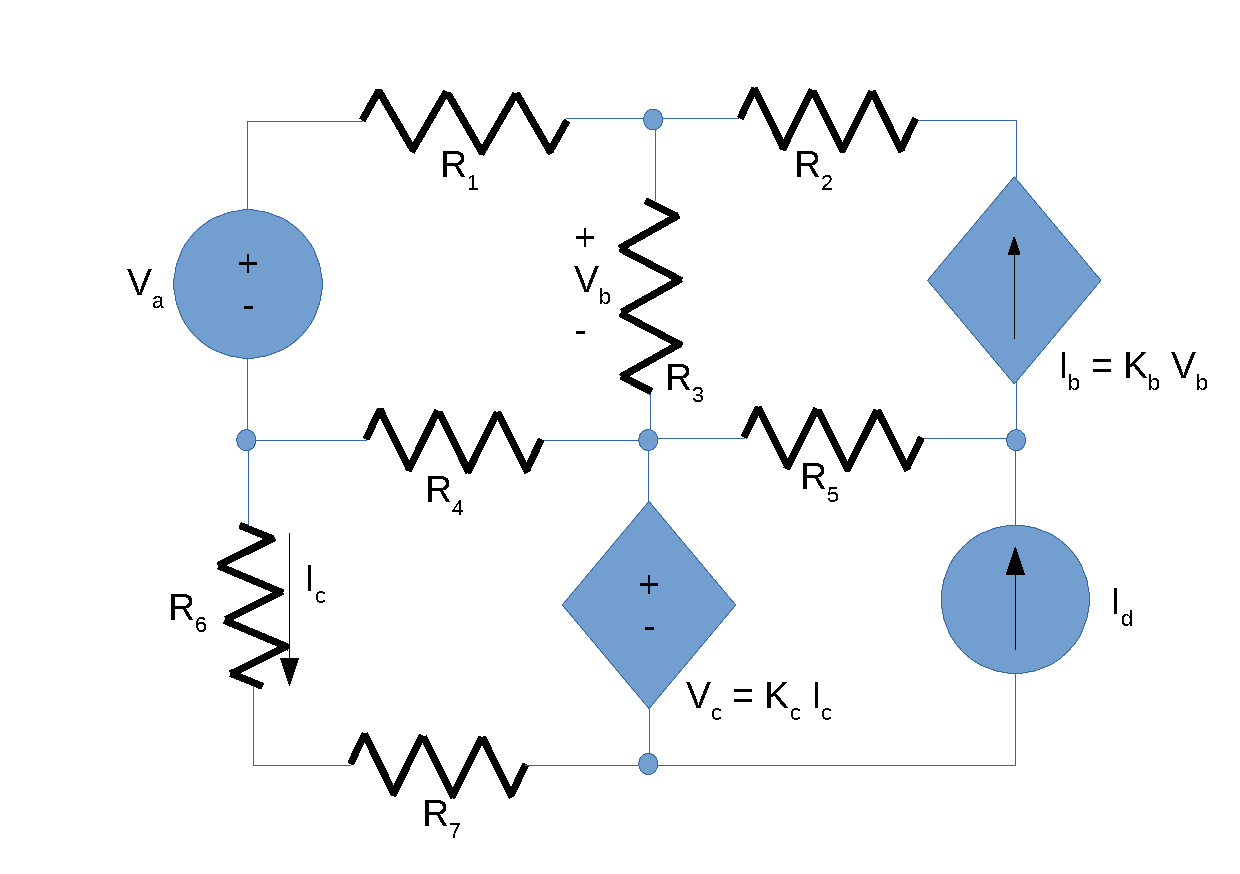
\includegraphics[width=0.6\linewidth]{simple.pdf}
%  \caption{Circuit considered}
%  \label{circuit}
%\end{figure}

